\documentclass[12pt, a4paper]{article}
\setlength{\parindent}{0pt}
\usepackage[a4paper, portrait, margin=1in]{geometry}
\usepackage{graphicx}

\graphicspath{.}

\usepackage{preamble}

\begin{document}

\textbf{Q1}

\textit{(a)} \textit{See combined sketch below.}

\textit{(b)} $F(0) = \int_{0}^{0} f(t) dt = 0$

\textit{(c)} $F(x)$ has critical points at -2, 0, and 1, by properties
of the derivative.

\textit{(d)} By properties of the derivative, $F(x)$ is increasing on
$(-2, 0)$ and for $x > 1$, and decreasing on $x < -2$ and $(0, 1)$.

\textit{(e)} By the second derivative, $F(x)$ is concave down for
$(\frac{-2 - \sqrt{28}}{6}, \frac{-2 + \sqrt{28}}{6})$ and
concave up everywhere else.

\textit{(f)}

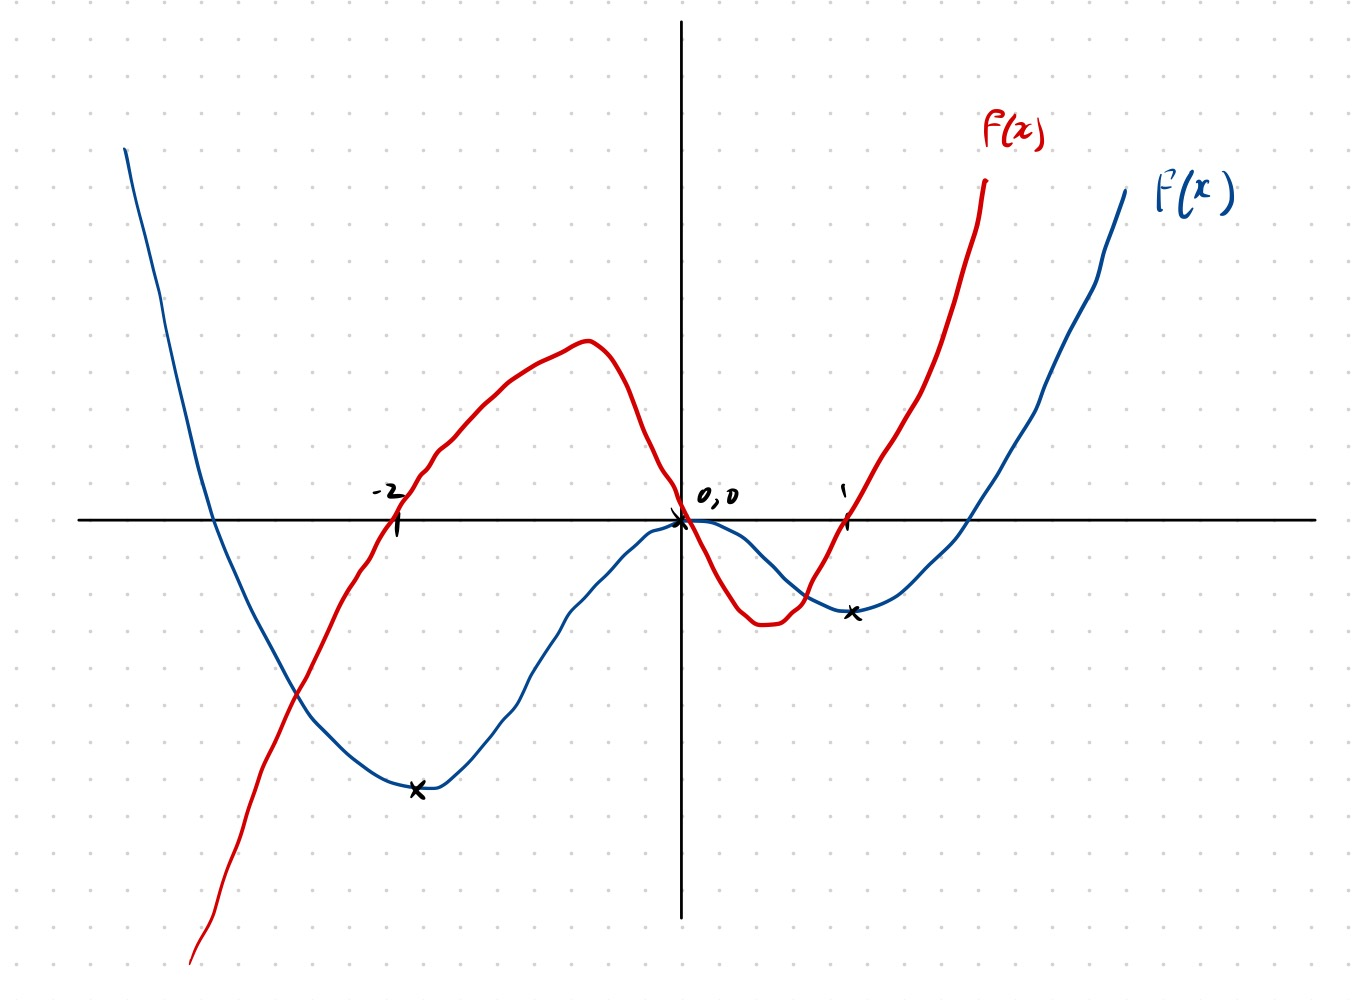
\includegraphics[width=\textwidth]{q1sketch.jpg}
\end{document}